%\documentclass[a4paper,
%%twocolumn
%]{article}
\documentclass[a4paper,9pt]{extarticle}

%%%%  Math
\usepackage{amsmath}
\DeclareMathOperator*{\argmin}{argmin}
\DeclareMathOperator*{\argmax}{argmax}
\newcommand*{\argminl}{\argmin\limits}
\newcommand*{\argmaxl}{\argmax\limits}

%%%%  Page margins
\usepackage{geometry}
%\geometry{left=25mm, right=20mm, top=30mm, bottom=20mm}
%\geometry{left=32mm, right=29mm, top=35mm, bottom=23mm}
\geometry{left=36mm, right=32mm, top=35mm, bottom=30mm}
%\geometry{left=15mm, right=15mm, top=25mm, bottom=20mm}
%\setlength{\columnsep}{4.5mm}

%%%% Configuration file for plotting
%%%%%%  Math
\usepackage{amsmath}
\usepackage{amssymb}

%%%%%%  Tables
\usepackage{booktabs}
% \usepackage{longtable}
\usepackage{multirow}
\usepackage{pgfplotstable}
\DeclareMathVersion{sansserif}
\SetSymbolFont{operators}{sansserif}{OT1}{cmss}{m}{n}
\usepackage{siunitx} 
\sisetup{group-separator={,}, group-minimum-digits={3}, parse-numbers=false}
\usepackage{tabularx}
\usepackage{ltablex}
\usepackage{array}
\newcolumntype{P}{>{\raggedleft\arraybackslash}p{.2in}}
\newcommand*{\dsSizeInTable}{\footnotesize}
\newcommand*{\unitSizeInTable}{\scriptsize}
\newcommand*{\tableSize}{\small}

%%%%%%  Figures
\usepackage{caption}
\usepackage{subcaption}
\captionsetup[subfigure]{position=bottom, labelfont=bf, textfont=normalfont, singlelinecheck=off, justification=raggedright}

%%%%%%  Figures in same page as they're called in twocolumn
\usepackage{stfloats}

%%%%%%  Balance columns of the last page in twocolumn environment
\usepackage{balance}

%%%%%%  Equations numbering format
\makeatletter
\renewcommand{\theequation}{S\arabic{equation}}
\def\tagform@#1{\maketag@@@{\bfseries(Eq.~\ignorespaces#1\unskip\@@italiccorr)}}
\makeatother

%%%%%%  Marks
\usepackage{pifont}
\newcommand{\xmark}{\ding{53}\xspace}%
\newcommand{\fmark}{\ding{110}\xspace}%

%%%%%  Color
\usepackage{xcolor}
%\newcommand*{\highlight}[1]{\textcolor{red}{\textbf{#1}}}
\newcommand*{\highlight}[1]{\textcolor{red!90!black}{#1}}
%\usepackage{easyReview}
%\usepackage{soul}  % Highlight command \hl
%\newcommand{\highlight}[1]{\hl{#1}}


%%%%%  Figures path
\usepackage{graphicx}
\graphicspath{{./fig/}}

%%%%%  Code styles
\usepackage{listings}
\lstset{
%	language=bash,
	basicstyle=\ttfamily,
	backgroundcolor=\color{black!5},
	commentstyle=\color{green!50!black},
	showstringspaces=false,
	numbers=left,
	numberstyle=\footnotesize\sffamily\color{gray!50},
	breaklines=true,
	mathescape=false %,
	% literate={\$}{{\$}}1
}
\lstdefinestyle{bash}{
	language=bash,
	basicstyle=\small\ttfamily,
}
\lstdefinestyle{cpp}{
	language=C++,
	basicstyle=\small\ttfamily,
}

%%%%%  Algorithms
\usepackage{algorithm}
\usepackage{algpseudocode}
\algnewcommand{\Inputs}[1]{%
  \State \textbf{Inputs:}
  \Statex \hspace*{\algorithmicindent}\parbox[t]{.8\linewidth}{\raggedright #1}
}
\renewcommand{\algorithmicrequire}{\textbf{Input:}}
\renewcommand{\algorithmicensure}{\textbf{Output:}}

%%%%%  Captions
\usepackage[figurename=Fig., tablename=Table, labelfont=bf, labelsep=period, font=small]{caption}
\renewcommand{\thefigure}{S\arabic{figure}}
\renewcommand{\thetable}{S\arabic{table}}

%%%%%  Links
\usepackage{hyperref}

%%%%%  Cites
\usepackage{cite}

%%%%%  Section, ... style
\usepackage{titlesec,titletoc}
\renewcommand*{\thesection}{S\arabic{section}}
\makeatletter
\renewcommand{\@seccntformat}[1]{%
	\ifcsname prefix@#1\endcsname
	\csname prefix@#1\endcsname
	\else
	\csname the#1\endcsname\quad
	\fi%
}
\newcommand\prefix@section{Note~\thesection\quad}
\makeatother
\titleformat*{\section}{\sffamily\Large\bfseries}
\titleformat*{\subsection}{\sffamily\large\bfseries}
\titleformat*{\subsubsection}{\sffamily\bfseries}
\titlecontents{section}[2.1em]{\addvspace{3mm}}{\bfseries\contentslabel{1.8em}}{\hspace*{-2.3em}}{\titlerule*[1pc]{}\bfseries\contentspage}
\dottedcontents{subsection}[4.9em]{}{2.8em}{1pc}

%%%%%  Line spacing
\usepackage{setspace}
\newcommand*{\defaultLineSpace}{\setstretch{1.15}}
\newcommand*{\codeLineSpace}{\setstretch{1.1}}
\newcommand*{\refLineSpace}{\setstretch{1}}

%%%%%  Handle spaces
\usepackage{xspace}

%%%%%  Trademark, registerd mark
\usepackage{textcomp}

%%%%%  User-defined commands
\newcommand*{\method}[1]{\text{#1}\xspace}
\newcommand*{\smashpp}   {\method{Smash++}}
\newcommand*{\gzip}      {\method{gzip}}
\newcommand*{\Gzip}      {\method{gzip}}
\newcommand*{\bzip}      {\method{bzip2}}
\newcommand*{\Bzip}      {\method{bzip2}}
\newcommand*{\mfcompress}{\method{MFCompress}}
\newcommand*{\Mfcompress}{\method{MFCompress}}
\newcommand*{\deliminate}{\method{DELIMINATE}}
\newcommand*{\Deliminate}{\method{DELIMINATE}}
\newcommand*{\fqzcomp}   {\method{fqzcomp}}
\newcommand*{\Fqzcomp}   {\method{Fqzcomp}}
\newcommand*{\quip}      {\method{Quip}}
\newcommand*{\Quip}      {\method{Quip}}
\newcommand*{\dsrc}      {\method{DSRC~2}}
\newcommand*{\Dsrc}      {\method{DSRC~2}}
\newcommand*{\fqc}       {\method{FQC}}
\newcommand*{\Fqc}       {\method{FQC}}
\newcommand*{\aes}		   {\method{AES}}
\newcommand*{\Aes}		   {\method{AES}}
\newcommand*{\aescrypt}  {\method{AES~Crypt}}
\newcommand*{\Aescrypt}  {\method{AES~Crypt}}
\newcommand*{\szip}      {\method{7zip}}
\newcommand*{\cmake}     {\method{cmake}}
\newcommand*{\Cmake}     {\method{Cmake}}
\newcommand*{\xs}		     {\method{XS}}
\newcommand*{\Xs}		     {\method{XS}}
\newcommand*{\goose}	   {\method{GOOSE}}
\newcommand*{\Goose}	   {\method{GOOSE}}
\newcommand*{\fasta}     {FASTA\xspace}
\newcommand*{\Fasta}     {FASTA\xspace}
\newcommand*{\fastq}     {FASTQ\xspace}
\newcommand*{\Fastq}     {FASTQ\xspace}
\newcommand*{\sam}       {SAM\xspace}
\newcommand*{\Sam}       {SAM\xspace}
\newcommand*{\bam}       {BAM\xspace}
\newcommand*{\Bam}       {BAM\xspace}
\newcommand*{\sambam}    {SAM/BAM\xspace}
\newcommand*{\Sambam}    {SAM/BAM\xspace}
\newcommand*{\vcf}       {VCF\xspace}
\newcommand*{\Vcf}       {VCF\xspace}
\newcommand*{\linux}     {Linux\xspace}
\newcommand*{\Linux}     {Linux\xspace}
\newcommand*{\windows}   {Windows\xspace}
\newcommand*{\Windows}   {Windows\xspace}
\newcommand*{\macos}     {macOS\xspace}
\newcommand*{\Macos}     {macOS\xspace}
\newcommand*{\xor}       {XOR\xspace}

\newcommand*{\sym}[1]{\text{#1}\xspace}
\newcommand*{\symA}      {\sym{A}}
\newcommand*{\symC}      {\sym{C}}
\newcommand*{\symG}      {\sym{G}}
\newcommand*{\symT}      {\sym{T}}
\newcommand*{\symN}      {\sym{N}}
\newcommand*{\symX}      {\sym{X}}

\newcommand*{\ascii}     {\mbox{ASCII}\xspace}

\newcommand*{\mono}[1]{\lstinline|#1|}
\newcommand*{\lang}[1]{\mono{#1}\xspace}
\newcommand*{\cpp}       {\lang{C++}}
\newcommand*{\bash}      {\lang{bash}}

%%%%%  User-defined environments
\lstnewenvironment{code}[1][]
	{\codeLineSpace\lstset{#1}\bgroup}
	{\egroup\defaultLineSpace}

%%%%  Headers and footers
\usepackage{fancyhdr}
\pagestyle{fancy}
\renewcommand{\sectionmark}[1]{\markright{Note~\thesection. #1}}
\renewcommand{\subsectionmark}[1]{\markright{\thesubsection. #1}}
\fancyhead{}    % clear all header fields
\fancyfoot{}    % clear all footer fields
\fancyhead[L]{\textsf{\nouppercase\rightmark}}
\fancyhead[R]{\thepage}
\setlength{\headsep}{20pt}


\begin{document}

%%% Title page
\begin{titlepage}
  \centering
  \vspace*{10mm}
  % \includegraphics[width=2.8cm]{logo.png} \\[10mm]
  \Large\textsc{Supplementary Material for} \\[5mm]
  \huge\textbf{Smash++: finding rearrangements} \\[12mm]
  \Large Morteza Hosseini\textsuperscript{1}, Diogo Pratas\textsuperscript{1,2}, Armando J. Pinho\textsuperscript{1} \\[6mm]
  \normalsize \textsuperscript{1}IEETA/DETI, University of Aveiro, Portugal \\[1mm]\textsuperscript{2}Department of Virology, University of Helsinki, Finland \\[4mm]
  {\ttfamily\{seyedmorteza,pratas,ap\}@ua.pt}
  
  \vspace{\fill}
  \thispagestyle{empty}
  \raggedright
  \setstretch{1.2}
  \normalsize\tableofcontents
\end{titlepage}

\defaultLineSpace    		%%% Line spacing

\clearpage
\section{GGA 18 compared to MGA 20}
\begin{figure}[!h]
  \centering
  % \includegraphics[width=\linewidth]{fig/PXO99A_MAFF.png}
  \caption{adopted from \cite{}.}
  % \label{fig.schema}
\end{figure}

\clearpage
\section{PXO99\textsuperscript{A} compared to MAFF}
\begin{figure}[!h]
  \centering
  \includegraphics[width=\linewidth]{fig/PXO99A_MAFF.png}
  \caption{adopted from \cite{salzberg2008genome}.
    Inversions and rearrangements in PXO99A compared to MAFF. The alignment shows regions of PXO99A that align to the same (red) or opposite (blue) strand of MAFF. Transposase genes and their orientation (+ or -) are shown at the sites of each rearrangement. Letters A-J indicate specific rearrangement events. A: the IS element ISXoo3 is composed of two distinct and independently conserved ORFs and is responsible for an inversion spanning coordinates 267869–5114959 (all coordinates refer to the PXO99A genome). B: ISXo8 occurs in opposite orientation at each end of a 2.6 Mbp inversion spanning positions 1356757–3898472. C: ISXo1 occurs in inverted copies at the endpoints of a 1.8 Mbp inversion spanning 1558996–3391786. D: a 33270 bp inverted region spanning 4394742–4428012 is flanked by oppositely-oriented copies of ISXo8. E: Each copy of the 212-kb duplication is flanked by ISXo5, which also occurs adjacent to two other translocations in this region. The duplication appears as two parallel diagonal lines in this box. F: ISXo8 also occurs in inverted copies at the boundaries of a 47540 bp segment that is translocated from approximately 4800000 to 685272. G: ISXoo3 flanks both ends of a 47540 bp translocation from approximately 1117000 to 4339239. H: A 9,862 bp region occurs in inverted copies at 217,455 and 4,305,307. MAFF311018 contains only one copy of this region. I,J: Segments spanning 96,753 bp (I) and 17,021 bp (J) are inverted with respect to MAFF311018 but not associated with transposases.}
  % \label{fig.schema}
\end{figure}

\clearpage
\section{Tool availability and implementation}
\label{sec.tool}
\smashpp is implemented in \cpp language and is available at~\cite{web-smashpp}. This tool is able to find and visualize rearrangements in sequences, \fasta and \fastq files; although, it is highly recommended to use sequences as input. In the following sections, we describe installing and running the \smashpp tool.

\subsection{Install}
To install \smashpp on various operating systems, follow the instructions below. Note that the precompiled executables are available for 64 bit operating systems in the ``bin/'' directory.

% \paragraph{Conda}
% % todo

\subsubsection*{Linux}
\begin{itemize}
  \item Install ``git'' and ``cmake'':
\begin{code}[style=bash]
sudo apt update
sudo apt install git cmake
\end{code}
\item Clone \smashpp and install it:
\begin{code}[style=bash]
git clone https://github.com/smortezah/smashpp.git
cd smashpp
./install.sh
\end{code}
\end{itemize}

\subsubsection*{macOS}
\begin{itemize}
    \item Install ``Homebrew'', ``git'' and ``cmake'':
\begin{code}[style=bash]
/usr/bin/ruby -e "$(curl -fsSL https://raw.githubusercontent.com/Homebrew/install/master/install)"
brew install git cmake
\end{code}
\item Clone \smashpp and install it:
\begin{code}[style=bash]
git clone https://github.com/smortezah/smashpp.git
cd smashpp
./install.sh
\end{code}
\end{itemize}

\subsubsection*{Windows}
\begin{itemize}
  \item Download and install ``CMake'', e.g., from https://github.com/Kitware/CMake/releases/\linebreak download/v3.14.4/cmake-3.14.4-win64-x64.msi. Make sure to add it to the system PATH. For example, if CMake is installed in ``C:\textbackslash Program Files'', add ``C:\textbackslash Program Files\textbackslash CMake\textbackslash bin'' to the system PATH.
  \item Download and install ``mingw-w64'', e.g., from https://sourceforge.net/projects/mingw-w64/\linebreak files/latest/download. Make sure to add it to the system PATH. For example, if it is installed in ``C:\textbackslash mingw-w64'', add ``C:\textbackslash mingw-w64\textbackslash mingw64\textbackslash bin'' to the system PATH.
  \item Download and install ``git'', from https://git-scm.com/download/win.
  \item Clone \smashpp and install it:
\begin{code}[style=bash]
git clone https://github.com/smortezah/smashpp.git
cd smashpp
.\install.bat
\end{code}
\end{itemize}

\subsection{Run \smashpp}
Various options are provided with the interface of the proposed tool, which are described in Table~\ref{tab.options}. The commands for running \smashpp have the form of the following:
\begin{code}[style=bash]
./smashpp [OPTIONS]  -r <REF-FILE>  -t <TAR-FILE>
\end{code}

\begin{small}
\begin{tabularx}{\linewidth}{@{}lp{2.95cm}X@{}}
  \caption{Options provided by \smashpp interface.}
  \label{tab.options} \\
  \toprule
  Flag & Input & Description \\
  \midrule
  \multicolumn{3}{@{}l@{}}{\textit{Required}} \\
  \mono{-r} & Seq/FASTA/FASTQ & Reference file. \\
  \mono{-t} & Seq/FASTA/FASTQ & Target file. \\
  && It is highly recommended to have short names. \\
  \midrule
  \multicolumn{3}{@{}l@{}}{\textit{Optional}} \\
  \mono{-l} & Integer: $[0, 5]$\newline Default: 0 & Level of compression. \\
  \midrule
  \mono{-m} & Integer: $[1, 2^{32}-1]$\newline Default: 50 & Minimum segment size. Only those regions in the reference file that are bigger than this value would be able to be considered for compression. \\
  \midrule
  \mono{-e} & Float: $[0.0, 100.0]$\newline Default: 2.0 & Entropy of `N's. In implementation of the reference-based compression, we have replaced `N' bases in the references and the targets with `A's and `T's, respectively. On reference-free compression, they are replaced with `A's, in both references and targets. If a user tends to replace `N' bases in a sequence with a normal distribution of `A', `C', `G' and `T's, he/she can employ GOOSE toolkit~\cite{web-goose}. \\
  \midrule
  \mono{-n} & Integer: $[1, 8]$\newline Default: 4 & Number of threads. Creating multiple finite-context models and substitutional-tolerant Markov models can be done in a multi-threaded fashion. \\
  \midrule
  \mono{-f} & Integer: $[1, 2^{32}-1]$\newline Default: 256 & Filter size. In the process of finding similar regions in the reference and the target sequences, the information content that would be obtained by compression needs to be filtered. \\
  \midrule
  \mono{-ft} & Integer or String:\newline \{0$\,|\,$rectangular, 1$\,|\,$hamming, 2$\,|\,$hann, 3$\,|\,$blackman, 4$\,|\,$triangular, 5$\,|\,$welch, 6$\,|\,$sine, 7$\,|\,$nuttall\}\newline Default: hann & Filter type (windowing function). Besides Hann window that is used by default to smooth the information content (profile), we have implemented several other windowing functions: Blackman~\cite{blackman1959particular}, Hamming~\cite{tukey1949measuring}, Nuttall~\cite{nuttall1981some}, rectangular~\cite{oppenheim1999discrete}, sine~\cite{harris1978use}, triangular~\cite{bartlett1950periodogram} and Welch~\cite{welch1967use} windows. These functions are given by Equation~\ref{eq.filter} and are plotted in Fig.~\ref{fig.filters}. \\
  \midrule
  \mono{-fs} & Char or String:\newline \{S$\,|\,$small, M$\,|\,$medium, L$\,|\,$large\}\newline Default: large & Filter scale. Automatically chooses filter size. \\
  \midrule
  \mono{-d} & Integer: $[1, 2^{64}-1]$\newline Default: 1 & Sampling steps. Instead of considering the whole information content, this option can be used to make samples of it. \\
  \midrule
  \mono{-th} & Float: $[0.0, 20.0]$\newline Default: 1.5 & threshold. For the purpose of segmenting the filtered information content, the average entropy of reference-based compression is used by default as the threshold, but the threshold can be altered by this option. \\
  \midrule
  \mono{-rb} & Integer: $[-2^{15}, 2^{15}-1]$ & Reference beginning guard. \\
  \mono{-re} & Integer: $[-2^{15}, 2^{15}-1]$ & Reference ending guard. \\
  \mono{-tb} & Integer: $[-2^{15}, 2^{15}-1]$ & Target beginning guard. \\
  \mono{-te} & Integer: $[-2^{15}, 2^{15}-1]$ & Target ending guard. \\
  & Default: 0 & \smashpp is capable of finding even very small similar regions in two sequences. However, we have found experimentally that when it is running in a very sensitive mode, there might be some cases in which the size of similar regions in the reference and the target are not balanced. These cases can be handled by ``-rb'', ``-re'', ``-tb'' and ``-te'' options, that can resize the beginning and ending guards of reference and target regions, respectively. For example, if ``-tb 10'' is used, the first 10 bases in each target region will be ignored, which results in smaller regions. Note that when the guard sizes of target regions are increased, the models built from these regions would be slightly different than the original models; consequently, the sizes of reference regions that are detected as being similar to the ones from the target would be modified, as well. Therefore, changing the guard sizes of target regions will affect the sizes of reference regions. In the case of activating deep compression, by ``-dp'', changing the guard sizes of reference regions would affect the sizes of target regions, as well. \\
  \midrule
  \mono{-dp} & --- & Deep compression. The ``deep compression'' means that similar regions in target and reference sequences are found in three phases instead of two: 1) the model of the reference is built and the target is compressed based upon that model, 2) the model of each detected region is built and the whole reference is compressed based on these models and 3) the model of each detected reference region is built and the corresponding target regions will be compressed based on that model. \\
  \midrule
  \mono{-nr} & --- & Do not compute self complexity. It makes the tool not to perform the reference-free compression (self-complexity computation). \\
  \midrule
  \mono{-sb} & --- & Save sequence (input: FASTA/FASTQ). \smashpp accepts \fasta and \fastq files as input, in addition to sequences. In these cases, the input files are first converted to sequences and then processed further. It is possible to save these sequences by this option. \\
  \midrule
  \mono{-sp} & --- & Save profile, *.prf. When the information profile is obtained, \smashpp smoothens then removes it by default. However, it can be preserved by this option. \\
  \midrule
  \mono{-sf} & --- & Save filtered file, *.fil. The filtered profile is segmented then removed, by default; however, it can be preserved by this option. \\
  \midrule
  \mono{-ss} & --- & Save segmented files, *.s$_i$. \\
  \midrule
  \mono{-sa} & --- & Save profile, filtered and segmented files. \\
  \midrule
  \mono{-rm} & $k$,[$w$,$d$,]ir,$\alpha$,$\gamma$/$t$,ir,$\alpha$,$\gamma$:... & Parameters of reference models. \\
  \mono{-tm} & $k$,[$w$,$d$,]ir,$\alpha$,$\gamma$/$t$,ir,$\alpha$,$\gamma$:... & Parameters of target models: \\
& Default: $14,0,0.005,0.95$ & \begin{minipage} [t] {9cm}
  \begin{itemize}
    \item $k$ (integer $>1$): context size,
    \item $w$ (integer $<2^{64}-1$): sketch width in $\log_2$ form, e.g., set 10 for $w=2^{10}=1024$,
    \item $d$ (integer $>0$): sketch depth,
    \item ir (integer: \{0, 1, 2\}): inverted repeat, including 0:~regular (not inverted), 1:~inverted solely, and 2:~both regular and inverted,
    \item $\alpha$ (float $>0$): estimator,
    \item $\gamma$ (float: $[0.0, 1.0)$): forgetting factor,
    \item $t$ (integer $>0$): threshold (number of substitutions).
  \end{itemize}
\end{minipage} \\
  && It is recommended for compression to use ``-l'' option, since it configures the models automatically. However, using ``-rm'' and ``-tm'', the user would be able to manually configure the reference model, for reference-based compression, and the target model, for reference-free compression, respectively. Parameters of the models are described in detail in section~\ref{sec.methods}. \\
  \midrule
  \mono{-ll} & --- & Show list of parameters that would be chosen automatically for each model. \\
  \midrule
  \mono{-h} & --- & Usage guide. \\
  \midrule
  \mono{-v} & --- & More information (verbose). \\
  \midrule
  \multicolumn{2}{@{}l}{\mono{--version}} & Show version. \\
  \bottomrule
\end{tabularx}
\end{small}

\begin{align}
  w[n] & = 1,
  \tag*{(rectangular)}                                                                                                                                        \\
  w[n] & = 1-\left|\tfrac {n-N/2}{L/2}\right|, \quad L=N,
  \tag*{(triangular/Bartlett)}                                                                                                                                \\
  w[n] & = 1-\left(\tfrac {n-N/2}{N/2}\right)^{2},
  \tag*{(Welch)}                                                                                                                                              \\
  w[n] & = \sin \left(\tfrac {\pi n}{N}\right),
  \tag*{(sine)}                                                                                                                                               \\
  w[n] & = 0.54348-0.45652\;\cos \left(\tfrac {2\pi n}{N}\right),
  \tag*{(Hamming)}                                                                                                                                            \\
  w[n] & = 0.42659-0.49656\;\cos \left(\tfrac {2\pi n}{N}\right)+0.07685\;\cos \left(\tfrac {4\pi n}{N}\right),
  \tag*{(Blackman)}                                                                                                                                           \\
  w[n] & = 0.35577-0.48740\;\cos \left(\tfrac {2\pi n}{N}\right)+0.14423\;\cos \left(\tfrac {4\pi n}{N}\right)-0.01260\;\cos \left(\tfrac {6\pi n}{N}\right),
  \tag*{(Nuttall)}                                                                                                                                            \\
  \label{eq.filter}
\end{align}
\begin{figure}[!h]
  \centering
  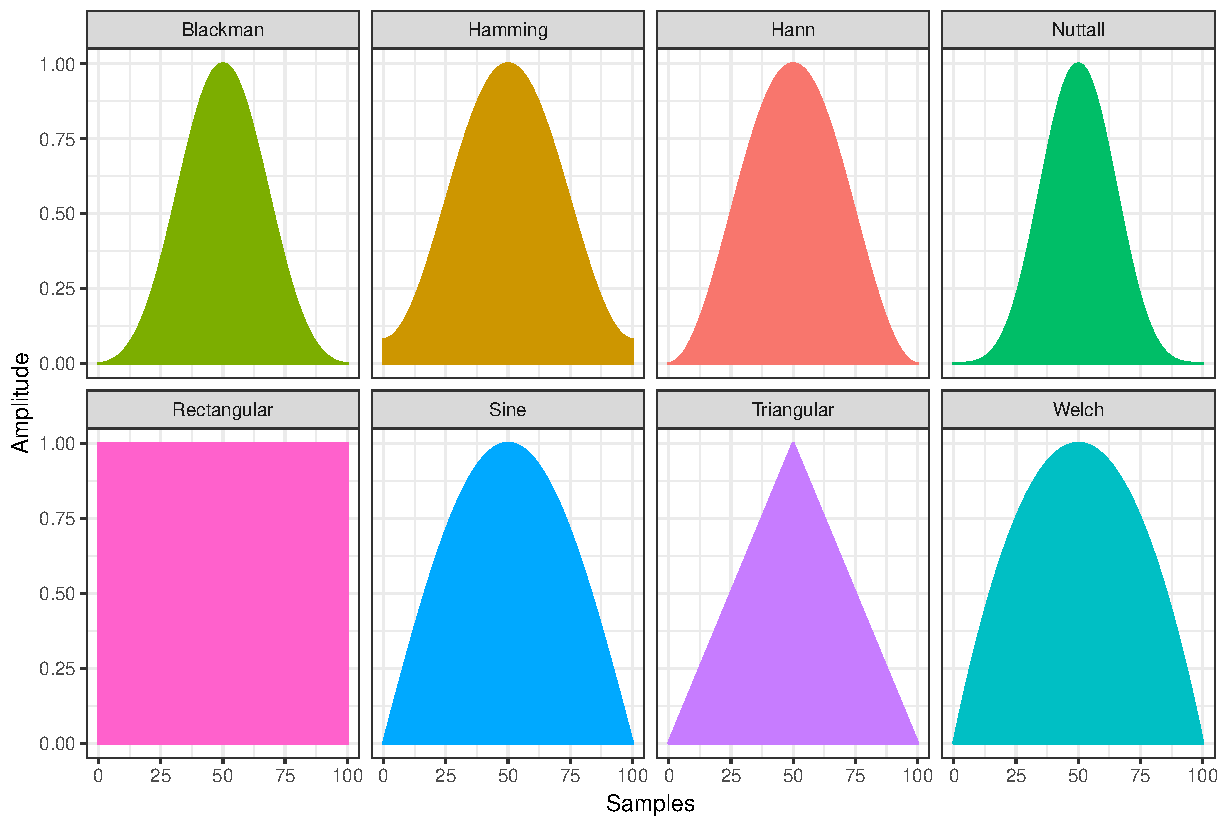
\includegraphics[width=\linewidth]{fig/filters.pdf}
  \caption{Various windowing functions implemented and embedded in \smashpp.}
  \label{fig.filters}
\end{figure}

By running \smashpp, positions of the similar regions in reference and target sequences, and also complexity of the regions is saved in a ``.pos'' file. This tab-separated file has a header including:
\begin{enumerate}
  \item The string ``\#SMASHPP'' as a specifier for the \smashpp tool,
  \item The name of reference sequence,
  \item The size of reference sequence,
  \item The name of target sequence,
  \item The size of target sequence,
\end{enumerate}
and a body including:
\begin{enumerate}
  \item Initial position of the reference sequence,
  \item Final position of the reference sequence,
  \item Average entropy of compressing the associated target block considering this reference block as the reference,
  \item Complexity (average entropy) of the detected reference block, calculated by reference-free compression,
  \item Initial position of the target sequence,
  \item Final position of the target sequence,
  \item Average entropy of compressing the associated reference block considering this target block as the reference,
  \item Complexity of the detected target block, calculated by reference-free compression.
\end{enumerate}
As an example, the header of the following ``.pos'' file shows that the reference ``Ref'' and the target ``Tar'' are 5,000,000 bases long. The body shows that there is a block in the Ref, from the position 2000000 up to 3000000, which is similar to a block in the Tar, from the position 3000000 to 4000000. Average entropy of compressing the Tar block, using the Ref block as reference, is 0.255555. This number is 0.26666 when the Ref block is compressed based on the model of the Tar block. Also, complexities of the Ref and the Tar blocks are 1.97777 and 1.98888, respectively.
\begin{code}[style=bash]
#SMASHPP Ref      5000000  Tar      5000000
2000000	 3000000  0.26666  1.97777  3000000  4000000  0.25555 1.98888
\end{code}


\subsection{Run \smashpp visualizer}
The position file obtained by running \smashpp can be visualized by
\begin{code}[style=bash]
./smashpp -viz
\end{code}
The visualizer provides various options that are described in Table~\ref{tab.options.viz}. The commands for running \smashpp visualizer are of the form
\begin{code}[style=bash]
./smashpp -viz [OPTIONS]  -o <SVG-FILE>  <POS-FILE>
\end{code}

\begin{small}
  \begin{tabularx}{\linewidth}{@{}lp{2.7cm}X@{}}
    \caption{Options provided by \smashpp visualizer interface.}
    \label{tab.options.viz} \\
    \toprule
    Flag & Input & Description \\
    \midrule
    \multicolumn{3}{@{}l@{}}{\textit{Required}} \\
    & *.pos file & Position file, generated by Smash++ tool. \\
    \midrule
    \multicolumn{3}{@{}l@{}}{\textit{Optional}} \\
    \mono{-o} & *.svg file\newline Default: map.svg & Output image name. \\
    \midrule
    \mono{-rn} & String & Reference name shown on output. \\
    \mono{-tn} & String & Target name shown on output. \\
    & Default: names in position file's header & If it has space, use double quotes, e.g. ``Seq label''. \\
    \midrule
    \mono{-l} & Integer: $[1, 6]$\newline Default: 1 & Type of the link between maps. \\
    \midrule
    \mono{-c} & Integer: $[0, 1]$\newline Default: 0 & Color mode. \\
    \midrule
    \mono{-p} & Float: $[0.0, 1.0]$\newline Default: 0.9 & Opacity. \\
    \midrule
    \mono{-w} & Integer: $[15, 100]$\newline Default: 16 & Width of the sequence. \\
    \midrule
    \mono{-s} & Integer: $[15, 200]$\newline Default: 62 & Space between sequences. \\
    \midrule
    \mono{-f} & Integer: $[1, 255]$\newline Default: 43 & Multiplication factor for color ID. \\
    \midrule
    \mono{-b} & Integer: $[0, 255]$\newline Default: 0 & Beginning of color ID. \\
    \midrule
    \mono{-rt} & Integer: $[1, 2^{32}-1]$ & Reference tick size. \\
    \mono{-tt} & Integer: $[1, 2^{32}-1]$ & Target tick size. \\
    \midrule
    \mono{-th} & Integer: $\{0, 1\}$\newline Default: 1 & Tick human readable: 0=false, 1=true. If it is true, the sizes on axes are printed in the format 1K, 2M, etc. Note that here, 1K is equivalent to 1000 and not 1024, and so on. \\
    \midrule
    \mono{-m} & Integer: $[1, 2^{32}-1]$\newline Default: 1 & Minimum block size. Only the regions that are bigger than this value will be illustrated. \\
    \midrule
    \mono{-vv} & --- & Vertical view of the output image. \\
    \midrule
    \mono{-nn} & --- & Do not show normalized relative compression (NRC). \\
    \mono{-nr} & --- & Do not show self complexity. \\
    && \smashpp performs reference-based and reference-free compressions to calculate the NRC and redundancy (self complexity), respectively. If the user is not interested in showing them, he/she can turn them off by ``-nn'' and ``-nr'' triggers. \\
    \midrule
    \mono{-ni} & --- & Do not show inverse maps. \\
    \mono{-ng} & --- & Do not show regular (not inverse) maps. \\
    && \smashpp considers by default both regular and reverse complement maps in its calculations. \\
    \midrule
    \mono{-h} & --- & Usage guide. \\
    \midrule
    \mono{-v} & --- & More information (verbose). \\
    \midrule
    \multicolumn{2}{@{}l@{}}{\mono{--version}} & Show version. \\
    \bottomrule
  \end{tabularx}
\end{small}

% which gives
% \begin{code}[style=bash]
% SYNOPSIS
%   ./smashpp -viz [OPTIONS]  -o <SVG-FILE>  <POS-FILE>

% OPTIONS
%   Required:
%   <POS-FILE>         = position file, generated by
%                        Smash++ tool (*.pos)

%   Optional:
%   -o  <SVG-FILE>     = output image name (*.svg)             -> map.svg
%   -rn <STRING>       = reference name shown on output. If it
%                        has space, use double quotes, e.g.
%                        "Seq label". Default: name in header
%                        of position file
%   -tn <STRING>       = target name shown on output
%   -l  <INT>          = type of the link between maps: [1, 6] -> 1
%   -c  <INT>          = color mode: [0, 1]                    -> 0
%   -p  <FLOAT>        = opacity: [0.0, 1.0]                   -> 0.9
%   -w  <INT>          = width of the sequence: [15, 100]      -> 16
%   -s  <INT>          = space between sequences: [15, 200]    -> 62
%   -f  <INT>          = multiplication factor for             -> 43
%                        color ID: [1, 255]
%   -b  <INT>          = beginning of color ID: [0, 255]       -> 0
%   -rt <INT>          = reference tick: [1, 4294967295]
%   -tt <INT>          = target tick: [1, 4294967295]
%   -th [0][1]         = tick human readable: 0=false, 1=true  -> 1
%   -m  <INT>          = minimum block size: [1, 4294967295]   -> 1
%   -vv                = vertical view                         -> no
%   -nn                = do NOT show normalized relative       -> no
%                        compression (NRC)
%   -nr                = do NOT show self complexity           -> no
%   -ni                = do NOT show inverse maps              -> no
%   -ng                = do NOT show regular maps              -> no
%   -h                 = usage guide
%   -v                 = more information
%   --version          = show version
% \end{code}

% The output of \smashpp visualizer is an ``SVG'' file whose name is determined by ``-o'' option. By default, it is named ``map.svg''. 
% Names of the reference and the target, which are going to be printed on the output image, can be altered by ``-rn'' and ``-tn'', respectively. They are by default the names written in the positions file. 

% Options ``-l'', ``-c'', ``-p'', ``-w'', ``-s'', ``-f'' and ``-b'' can be used to change the appearance of the image.

% Assigning integers to ``-rt'' and ``-tt'' options will change the tick sizes of the reference and the target, respectively. \smashpp prints the sizes on axes in human readable format, e.g., 1K, 2M, etc. However, it can be triggered by ``-th'' option. Note that, here, 1K is equivalent to 1000 and not 1024, and so on. 

% By setting ``-m'' to an integer value, only the regions that are bigger than that value will be illustrated.
% To have a vertical view of the image, instead of the default horizontal view, one can use ``-vv'' trigger.

% \smashpp performs reference-based and reference-free compressions to calculate the normalized relative compression (NRC) and redundancy (self complexity), respectively. If the user is not interested in showing them, he/she can turn them off by ``-nn'' and ``-nr'' triggers. In addition, \smashpp considers by default both regular and reverse complement maps in its calculations. Triggering ``-ni'' and ``-ng'' will stop showing inverted and regular maps, respectively.

\subsection{Example}
This section guides step-by-step employing \smashpp to find and visualize rearrangements in a sample genomic data. Note that the commands can be run on Linux and macOS, however, they are similar in Windows.

\subsubsection*{Install \smashpp and provide the required files}
First, install \smashpp:
\begin{code}[style=bash]
git clone https://github.com/smortezah/smashpp.git
cd smashpp
./install.sh
\end{code}
Then, copy \mono{smashpp} executable file into \mono{example/} directory and go to that directory:
\begin{code}[style=bash]
cp smashpp example/
cd example/
\end{code}
There is a 1000 byte reference sequence, named \mono{refs}, and a 1000 byte target sequence, named \mono{tars}, in this directory. Running
\begin{code}[style=bash]
./smashpp -r refs -t tars -f 45 -l 3
./smashpp -viz -p 1 -s 50 -w 15 refs.tars.pos
\end{code}
results in Fig.~\ref{fig.example}, which has been saved as ``map.svg''.

\begin{figure}[!h]
  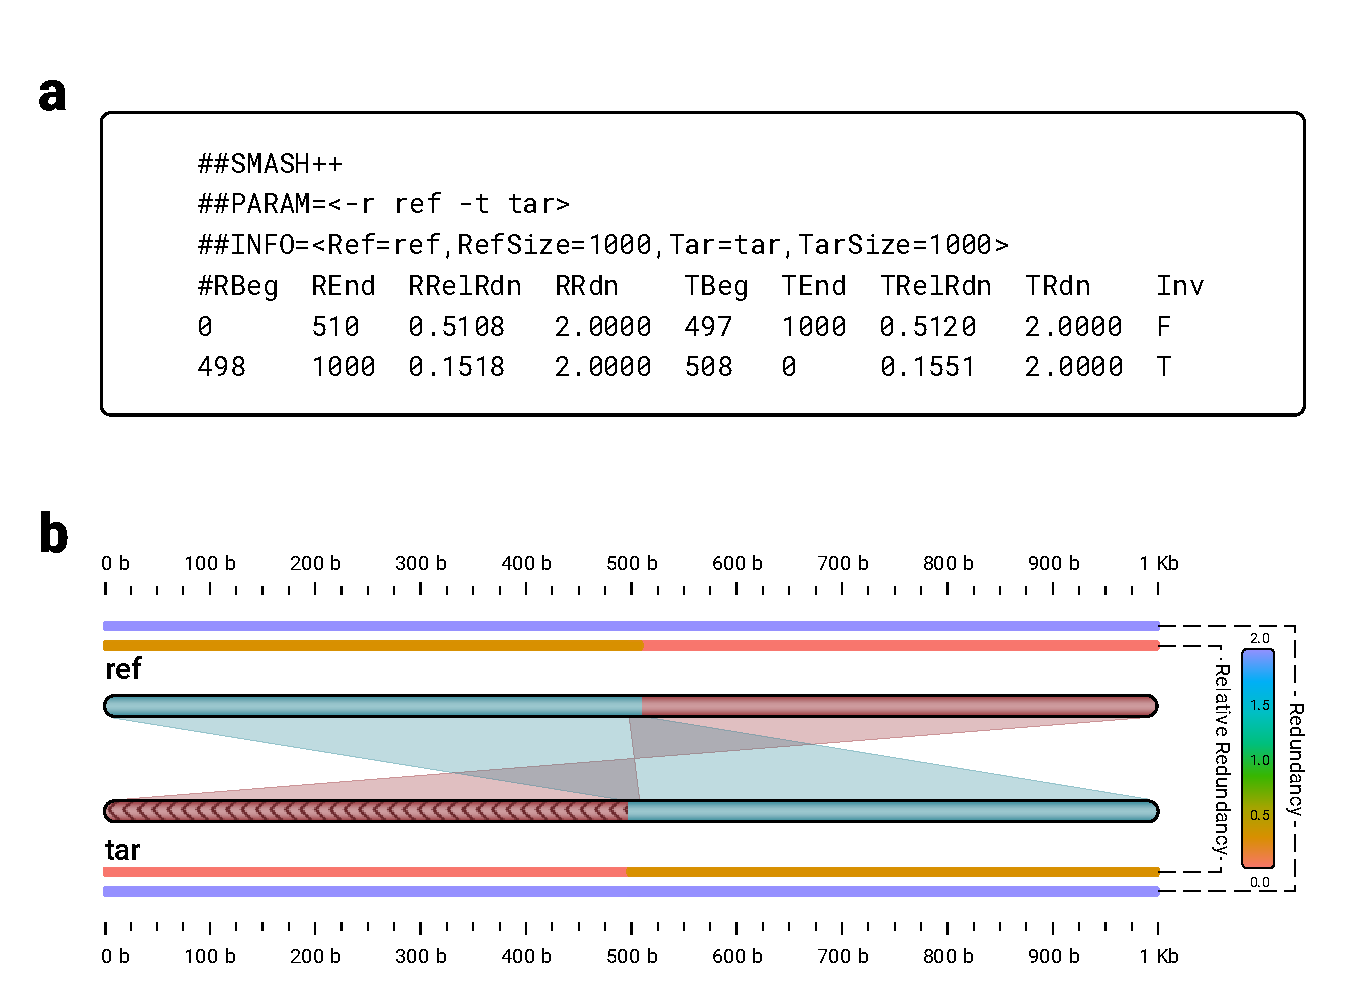
\includegraphics[width=.95\linewidth]{fig/example.pdf}
  \caption{An example of running \smashpp on two 1000 base sequences. Two similar regions in regular mode and two similar ones in inverted mode are detected.}
  \label{fig.example}
\end{figure}

\clearpage
%\balance
\refLineSpace    %%% Line spacing
\small
\addcontentsline{toc}{section}{\:\textbf{References}}
\bibliographystyle{IEEEtran}
\bibliography{ref}

\end{document}